\documentclass{article}
\usepackage{tikz} 
\usepackage{pgfplots} 
\usepackage{stix}
\usepackage{gillius}
\usepackage{ccicons}

\usepackage[margin=0in, includehead, includefoot, paperwidth=8.625in, paperheight=8.75in]{geometry}
\usetikzlibrary{backgrounds}
\usetikzlibrary{patterns}
\renewcommand{\d}{\mathop{}\!d}

\definecolor{scarlet}{RGB}{187,0,0}

\begin{document}
\pagenumbering{gobble}


\tikz[remember picture,overlay] \node[inner sep=0pt] at (current page.center){\includegraphics[height=8.75in]{starsBlue.jpg}};
%\tikz[remember picture,overlay] \node[inner sep=0pt] at (current page.center){\includegraphics[width=8.625in]{frontTemplate.png}};

\flushright

\begin{tikzpicture}[opacity=1]
  \node at (-.8,0) {\scalebox{4}{\Huge\textsf{\textbf{\textcolor{white}{calculus}}}}};
  \node at (8,1.19) {\scalebox{10}{\Huge\textsf{\textbf{\textcolor{white!65!black}{2}}}}};  %% Aligned with subtitle
  %\node at (8,1.85) {\scalebox{10}{\Huge\textsf{\textbf{\textcolor{white!65!black}{1}}}}}; %% Aligned with title
  \node at (-.7,-1.6) {\resizebox{4.8in}{.2in}{\Huge\textsf{\textcolor{white!65!black}
          {with free online interactive materials}
    }}};
    %\draw[yellow] (-9,-1.2)--(9,-1.2); %guide line
\end{tikzpicture}\hspace*{.3in}

\vspace{1in}


  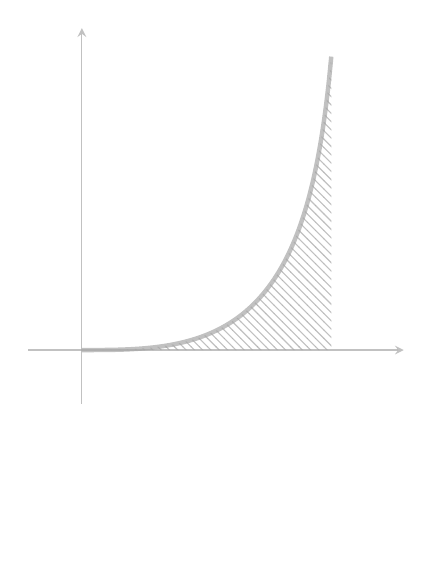
\begin{tikzpicture}[opacity =.7]
    \begin{axis}[
        xmin=-.2,
        xmax=1.2,
        ymin=-.4,
        ymax=2.4,
        width=2.5in,
        height=2.5in,
        clip=false,
        axis lines=middle, %xlabel=$x$, ylabel=$y$,
        every axis y label/.style={white!65!black,at=(current axis.above origin),anchor=south},
        every axis x label/.style={white!65!black,at=(current axis.right of origin),anchor=west},
        ticks=none,
        axis line style={white!65!black},
      ]
      \addplot [samples = 100,draw=none, domain=0:.93,smooth,pattern=north west lines, pattern color=white!65!black] {x^3/sqrt(1-x^2)}\closedcycle;
      \addplot [samples = 100,ultra thick, domain=0:.93,smooth,draw=white!65!black] {x^3/sqrt(1-x^2)};
      \node[white] at (axis cs: .5,-1) {\scalebox{1.2}{$\displaystyle\int_0^1 \frac{x^3}{\sqrt{1-x^2}}\d x$}};
    \end{axis}
  \end{tikzpicture}
  \hspace*{.6in}
  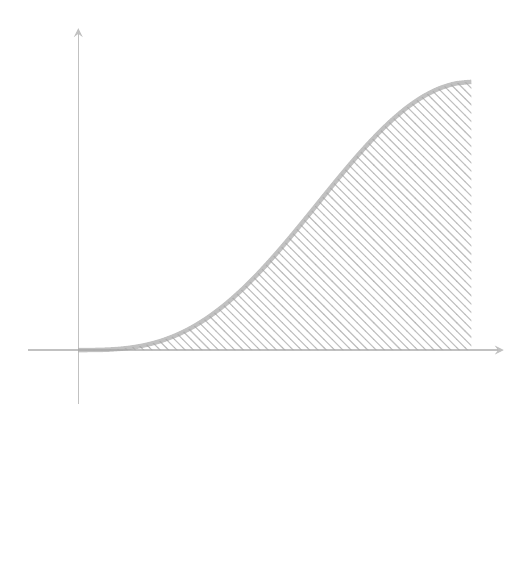
\begin{tikzpicture}[opacity =.7]
  \begin{axis}[
        xmin=-.2,
        xmax=1.7,
        ymin=-.2,
        ymax=1.2,
        width=3in,
        height=2.5in,
        clip=false,
        axis lines=middle, %xlabel=$x$, ylabel=$y$,
        every axis y label/.style={white!65!black,at=(current axis.above origin),anchor=south},
        every axis x label/.style={white!65!black,at=(current axis.right of origin),anchor=west},
        ticks=none,
        axis line style={white!65!black},
      ]
    \addplot [domain=0:pi/2,smooth,draw=none,pattern=north west lines, pattern color=white!65!black] {sin(deg(x))^3}\closedcycle;
    \addplot [domain=0:pi/2,smooth,ultra thick, draw=white!65!black] {sin(deg(x))^3};
    \node[white] at (axis cs: .75,-.5) {\scalebox{1.2}{$\displaystyle\int_0^{\pi/2} \sin^3(\theta)\d \theta$}};
    \end{axis}
  \end{tikzpicture}\hspace*{.6in}
  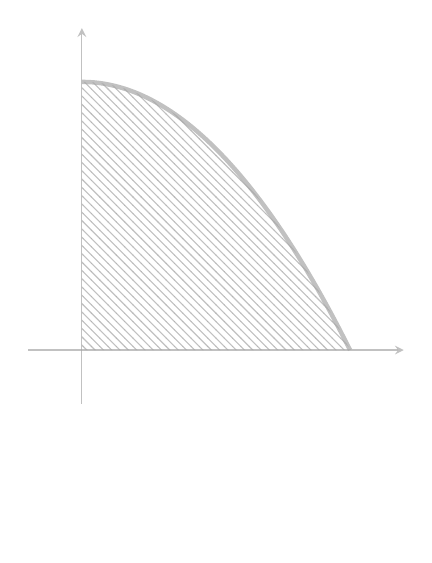
\begin{tikzpicture}[opacity =.7]
  \begin{axis}[
        xmin=-.2,
        xmax=1.2,
        ymin=-.2,
        ymax=1.2,
        width=2.5in,
        height=2.5in,
        clip=false,
        axis lines=middle, %xlabel=$x$, ylabel=$y$,
        every axis y label/.style={white!65!black,at=(current axis.above origin),anchor=south},
        every axis x label/.style={white!65!black,at=(current axis.right of origin),anchor=west},
        ticks=none,
        axis line style={white!65!black},
      ]
    \addplot [domain=0:1,smooth,draw=none,pattern=north west lines, pattern color=white!65!black] {1-x^2}\closedcycle;
    \addplot [domain=0:1,ultra thick,smooth,draw=white!65!black] {1-x^2};
    \node[white] at (axis cs: .5,-.5) {\scalebox{1.2}{$\displaystyle\int_0^{1} \left(g^2-1\right)\d g$}};

    \end{axis}
  \end{tikzpicture}\hspace*{.6in}

  \vfill


\flushleft
\hspace*{.4in}\begin{tikzpicture}
  \node at (0,0) {\scalebox{1}{\Huge\textsf{\textcolor{white}{\ccbyncsa}}}};
  \node at (4,-.2) {\large\textsf{\textcolor{white}{developed in \textbf{XIMERA}}}};
\end{tikzpicture}
\vspace*{.2cm}

\end{document}


